\documentclass{sciposter}
\usepackage{lipsum}
\usepackage{epsfig}
\usepackage{amsmath}
\usepackage{amssymb}
\usepackage{multicol}
\usepackage{graphicx,url}
\usepackage[portuges, brazil]{babel}  
\usepackage[utf8]{inputenc}
\usepackage{listings}
\usepackage{color}
\usepackage{indentfirst}

\lstset{language=C++,
                basicstyle=\ttfamily,
                keywordstyle=\color{blue}\ttfamily,
                stringstyle=\color{red}\ttfamily,
                commentstyle=\color{green}\ttfamily,
                morecomment=[l][\color{magenta}]{\#}
}
%\usepackage{fancybullets}
\newtheorem{Def}{Definition}


\title{Mini Games com \\ Visão Computacional}
%Título do projeto

\author{Gabriel Vieira Figueiredo Tomaz, Tales Carlos de Pádua, Vinicius de Carvalho}

\institute
{Bacharelado em Ciência da Computação\\
Centro Universitário SENAC - Campus Santo Amaro
  (SENAC-SP)\\
  Av. Engenheiro Eusébio Stevaux, 823 -- Santo Amaro, São Paulo -- CEP 04696-000 -- SP -- Brasil}
%Nome e endereço da Instituição

\email{vieira\_frifri@hotmail.com, talescpadua@gmail.com, carvalho.v@outlook.com}
% Onde você coloca os emails dos integrantes


%\date is unused by the current \maketitle

\rightlogo[1]{respect_cube}
\leftlogo[1]{Senac-logo}
% Exibe os logos (direita e esquerda)
% Procure usar arquivos png ou jpg, e de preferencia mantenha na mesma pasta do .tex
%%%%%%%%%%%%%%%%%%%%%%%%%%%%%%%%%%%%%%%%%%%%%%%%%%%%%%%%%%%%%%%%%%%%%%%%%%%%%%%%
%%% Begin of Document

\begin{document}
%define conference poster is presented at (appears as footer)

\conference{{\bf BCC 15 anos}, 5º Projeto Integrador III - 15 anos do Bacharelado em Ciência da Computação, Senac, 06 de Junho de 2014, São Paulo, Brasil}

%\LEFTSIDEfootlogo 
% Uncomment to put footer logo on left side, and
% conference name on right side of footer

% Some examples of caption control (remove % to check result)

%\renewcommand{\algorithmname}{Algoritme} % for Dutch

%\renewcommand{\mastercapstartstyle}[1]{\textit{\textbf{#1}}}
%\renewcommand{\algcapstartstyle}[1]{\textsc{\textbf{#1}}}
%\renewcommand{\algcapbodystyle}{\bfseries}
%\renewcommand{\thealgorithm}{\Roman{algorithm}}

\maketitle

%%% Begin of Multicols-Enviroment
\begin{multicols}{3}

%%% Abstract
\begin{abstract}
O projeto consiste em 2 jogos controlados por algoritmos de visão computacional, sendo que um deles tem a base voltada para identificação de cores primárias e o outro uma rústica detecção de face por meio de bordas e padrões de rosto.
\end{abstract}

%%% Introduction
\section{Introducão}
Jogos interativos tem sido uma grande área a ser explorada à medida que a tecnologia e as formas de se produzir jogos avançam. A partir disso, aliando-se do que a visão computacional tem a oferecer como ferramenta para a interface entre o humano e o computador, tem-se que este trabalho soma esses conceitos para criar uma jogabilidade diferente baseada interamente em câmeras de vídeo, de modo que este novo meio de interação intensifique a experiência do usuário.

\newcommand{\imsize}{0.45\columnwidth}


\section{Objetivos}
Visando abordar uma maior quantidade de conhecimentos na área de visão computacional, o grupo tomou como estratégia a criação de dois jogos com interfaces diferentes, um baseado na detecção de cores e o outro baseado na detecção de faces.

Para o primeiro jogo, o principal objetivo era reconhecer com precisão 4 cores básicas: verde, amarelo, azul e vermelho, de modo a estruturar o clássico jogo \textit{Genius}, que se basea em reconhecer estas cores descritas para validação de uma sequência correta de cores que o usuário deverá apresentar em frente à câmera.

O segundo jogo, um pouco mais complexo, envolve manipular as imagens vindas da câmera com o intuito de simplificar o que se está captando, sendo que, neste contexto, simplificar possibilita a detecção de certos padrões, como os de um rosto. Com o reconhecimento da face, o jogo se basea em um personagem dentro de um caminhão de sorvete utilizando o rosto para atender os pedidos de certos clientes.

\section{Metodologia}
No início do trabalho foi introduzido uma biblioteca, baseada em OpenCV, que faz a interface de acesso à câmera de maneira bem restrita, possibilitando apenas que houvesse contato com os quadros capturados da câmera fornecidos por uma matriz tridimensional onde a primeira dimensão é a altura (em pixels) da imagem, a segunda representa a largura (também em pixels) e a terceira são os componentes vermelho (red), verde (green) e azul (blue), respectivamente, do espaço de cores RGB. Todos os valores da matriz representam um número entre 0 e 255 do padrão RGB.

\subsubsection*{Jogo: Genius}

A principal ideia do reconhecimento das cores desse jogo foi o reconhecimento básico da cor vermelha, onde caso fosse verificado que o componente R da matriz fosse maior que a soma dos outros dois componentes, se tratava claramente da cor desejada. Apesar de funcionar relativamente bem para detecção de vermelho, as outras cores apresentavam uma resistência maior ao método devido a pequenas instabilidades e mudanças de luz, sendo necessário buscar algo mais sofisticado, como a utilização do espaço de cor HSV.

\subsubsection{Conversão de espaço de cor RGB para HSV}

A conversão do espaço de cor pode ser dada por:

\begin{figure}[ht]
\centering
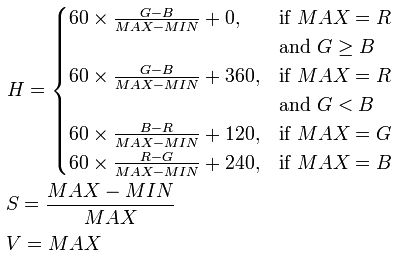
\includegraphics[width=8in]{img4.png}
\end{figure}

Neste espaço, cada ponto é representado por um conjunto HSV onde a componente H representa a cor propriamente dita, S a sua saturação e V o seu brilho. Com esta separação, ao contrário do que acontece no espaço RGB, pode-se facilmente determinar escopos (ranges) para cada cor, possibilitando assim uma filtragem mais precisa das cores desejadas.

\subsubsection*{Jogo: Sorvete Hoje?}

A ideia deste jogo surgiu a partir do estudo de certos algoritmos que aliados permitem uma detecção de borda, que foi a base para a detecção de face. A detecção desta borda é feita por meio do Filtro de Sobel, que será explicado mais adiante. Aliado ao filtro, para que houvessem bordas mais consistentes, foi utilizado um algoritmo de binarização de imagem. A técnica utilizada é conhecida como algoritmo de Otsu.

Apenas o filtro, porém, não era suficiente para atingir os objetivos, visto que a manipulação de quadros da câmera pode ser um processo bastante custoso, o que gera uma experiência ruim para o usuário. Visando um modo de se otimizar este processo, antes de se aplicar o algoritmo do filtro foi utilizada uma conversão da imagem para escala de cinza.

Por fim, para evitar impecilhos com a imagem de fundo da câmera, também foi agregado um algoritmo de remoção de fundo simples utilizando a fórmula matemática da Distância Euclidiana nos pixels dos quadros.

\subsubsection{Escala de Cinza}

O algoritmo de escala de cinza utilizado é bastante simples de ser aplicado no espaço de cor RGB, pois todos as cores obtidas ao se igualar as componentes R, G e B são tons de cinza. A fim de simplificar a quantidade de pixels que seriam processados, basta passar um algoritmo que soma as três componentes RGB de cada pixel, divide o valor por três e aplica o mesmo para as três componentes. Isto faz com que a imagem se torne descolorida com tons de cinza que são aproximações das cores da imagem original. Como as três componentes da terceira dimensão da matriz serão iguais, basta aplicar os algoritmos seguintes para apenas uma delas e replicar os resultados às demais, diminuindo assim a quantidade de processamento.

\subsubsection{Filtro de Sobel}

O Filtro de Sobel calcula o gradiente da intensidade da imagem em cada ponto, dando a direção da maior variação de claro para escuro e a quantidade de variação nessa direção por meio de duas matrizes quadradas de ordem 3, que são convoluídas com a imagem original para calcular aproximações das derivadas. Uma das matrizes representa a variação horizontal $Gx$ e a outra é a vertical $Gy$. \\

\begin{center}{Máscara de Sobel 3x3}
$$
Gx=\left[\begin{array}{rrr}
-1&0&+1\\
-2&0&+2 \\
-1&0&+1
\end{array}\right]\quad
Gy=\left[\begin{array}{ccc}
-1&-2&-1\\
0& 0& 0 \\
+1&+2&+1
\end{array}\right]
$$
\end{center}

E a partir disto, calcula-se a magnitude do gradiente:

$$
|G|=\sqrt{Gx^2 + Gy^2}
$$	

A variação de claro para escuro indica a presença de uma borda e com este gradiente aplicado nos canais RGB tem-se uma imagem composta apenas pelas bordas dos objetos que a compõem. Como a imagem utilizada está em escala de cinza, o resultado é uma imagem composta de bordas claras (próximas ao branco) com massas escuras (que tendem ao preto).

\subsubsection{Binarização da imagem}

Apesar dos diversos algoritmos para binarização de imagem, como os quadros que estão sendo trabalhados já estão bastante simplificados neste ponto, uma implementação baseada no algoritmo de Otsu é suficiente para atingir o objetivo de itensificar as bordas obtidas no Filtro de Sobel.

A ideia geral do método de Otsu é ter um valor limite onde se atribui a cor branca para os pixels que possuírem o canal RGB acima deste limite e preto para os que estiverem abaixo do mesmo. Essa limítrofe em geral é calculada a partir de fórmulas que utilizam a imagem para definir qual seria o valor mais adequado, entretanto, para a imagem com bordas, pode-se definir um valor constante e simplificar todo o processo.

\subsubsection{Remoção de fundo com Distância Euclidiana}

Quando se quer ignorar o fundo de um determinado cenário, pode-se aplicar a distância entre dois pontos definida por Euclides como $dist(p, q) = \sqrt{p^2 - q^2}$ onde p e q são pontos com cordenadas $p_{1}, p_{2}, ... p_{n}$ e $q_{1}, q_{2}, ... q_{n}$. Capturando um quadro da câmera onde não há nada além do fundo do cenário, basta iterar entre todos os pontos (pixels) p deste quadro e os pontos q do quadro que se deseja remover o fundo. O resultado é uma imagem que exclui, de maneira simples, os elementos do cenário.

\subsubsection{Detecção de rosto}
O resultado de todos estes algoritmos alinhados é uma imagem de bordas bem definidas composta apenas pelo que não faz parte do cenário capturado pela câmera, ou seja, na grande parte dos casos haverá apenas a borda detalhada do jogador. O usuário é então instruído a posicionar seu rosto em um local específico onde é feito o reconhecimento facial, baseando-se no fato de que são esperados muitos pixels brancos para os olhos e a boca, mas poucos para a face visto que não há muitas bordas na mesma.

\section{Resultados e Discussão}

Como resultado da conversão do espaço de cores HSV, a detecção das cores propostas ficou bastante consistente e permitiu a criação do jogo \textit{Genius} com sucesso, deixando apenas a necessidade de se aprender a trabalhar com o novo espaço de cor visto que ele pode não ser de aprendizado tão imediato quanto o RGB. Um exemplo de resultado com a detecção da cor azul:

\begin{figure}[ht]
\centering
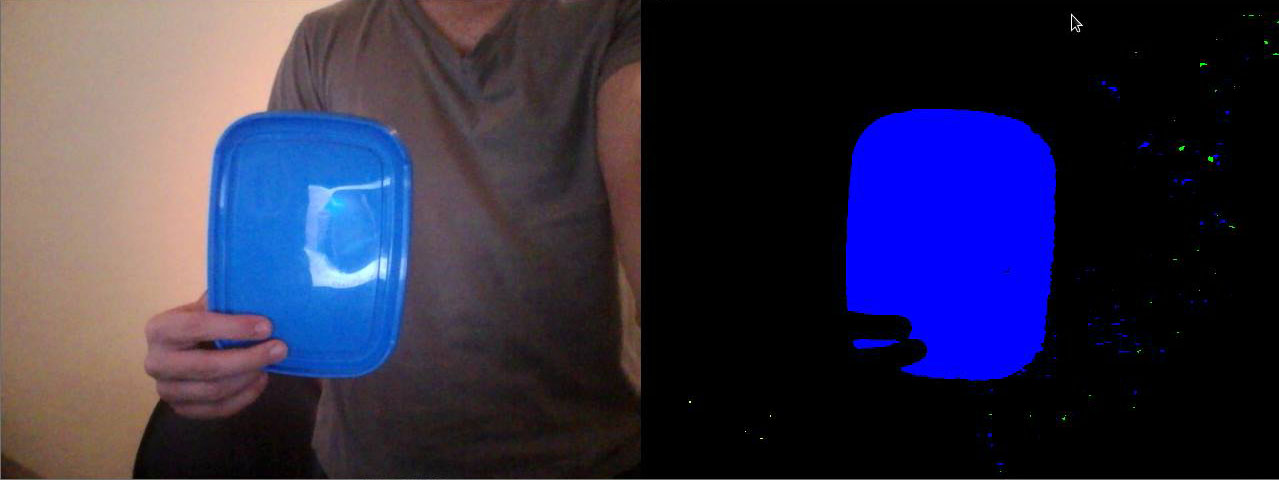
\includegraphics[width=8in]{img2.jpg}
\end{figure}

Já a detecção de rosto apresentou uma complexidade maior na elaboração, tendo a necessidade de se aliar diversos algoritmos para realizar uma detecção estável. Ela não funciona de forma perfeita mas é suficiente como interface de controle para o jogo \textit{Sorvete Hoje?}. A figura a seguir ilustra o resultado dos algoritmos descritos:

\begin{figure}[ht]
\centering
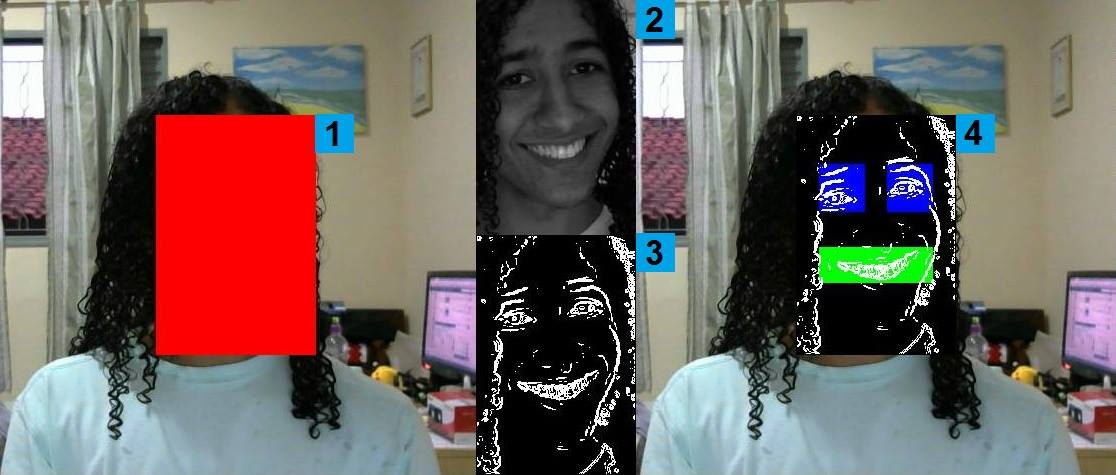
\includegraphics[width=8in]{img5.jpg}
\end{figure}

À esquerda está a imagem original da câmera com um retângulo vermelho no item 1 indicando onde está a face do jogador.
O item 2 representa a face do jogador em escala de cinza antes de ser aplicado o Filtro de Sobel, e o item 3 representa o mesmo após a aplicação do filtro e da binarização.
O item 4 representa uma máscara que indica o local onde espera-se que o usuário posicione o rosto para que seja feito o reconhecimento do mesmo.

\section{Conclusão}

Existem diversas formas de se trabalhar com visão computacional e mesmo limitando o escopo de trabalho para produzir apenas jogos, foi possível estudar e aplicar conceitos bastante diferentes entre si, como mudanças de espaço de cor e métodos de tratamento de imagem para reconhecimento de padrões. Apesar de não serem as técnicas mais sofisticadas, todos os algoritmos descritos atenderam as necessidades de cada jogo e assim foi possível criar uma experiência de usuário realmente inovadora tanto para um jogo clássico, como o \textit{Genius}, quanto para um jogo independente, como o caso do \textit{Sorvete Hoje?}. 
%%% References

%% Note: use of BibTeX als works!!

\bibliographystyle{plain}
\begin{thebibliography}{1}

%\bibitem{Flusser:Suk:93}
%J.~Flusser and T.~Suk.
%\newblock Pattern recognition by affine moment invariants.
%\newblock {\em Pattern Recognition}, 26:167--174, 1993.

  
%referencia do sobel
\bibitem{Sobel1968}
{SOBEL, Irvin}
\newblock A 3x3 isotropic gradient operator for image processing.
\newblock Never published but presented at a talk at the Stanford Artificial
  Project, 1968.
\end{thebibliography}

\end{multicols}

\end{document}